\chapter{Projetos de novas instalações produtivas (localização, capacidade e rede de operações)} 
\label{chap:projetos_de_novas} 

\section{Cadeia de suprimentos: estrutura, verticalização e terceirização} 
\label{sec:projetos_de_novas_supply_chain} 
A cadeia de suprimentos de um processo produtivo é a relação da empresa com seus fornecedores e clientes, e a relação destes com seus fornecedores e clientes como descrita na Figura \ref{fig:supply_chain}. Nesta figura é possível perceber que os fornecedores que lidam diretamente com a operação são os de primeira camada, e os fornecedores dos fornecedores compõem a segunda camada, e estes fazem parte da montante do processo. Igualmente para o lado jusante, que tem os clientes de primeira camada, contato direto com a operação, e clientes dos clientes, que são os de segunda camada.
\par Além disso nota-se que fornecedores e clientes de primeira camada fazem parte da rede imediata de fornecimento, e a rede completa é chamada de rede total de suprimentos.


\begin{figure}[H]
    \centering
    \caption{Cadeia de Suprimentos (supply chain)}
    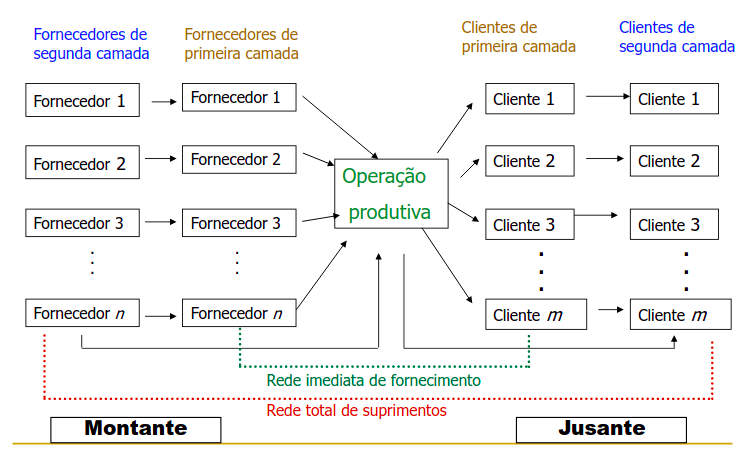
\includegraphics[scale=0.65]{images/supply_chain.png}
    \caption*{Fonte: \cite{supplychain}}
    \label{fig:supply_chain}
\end{figure}
  
\par A importância de entender toda a rede é vital para a competitividade da empresa devido aos seguintes aspectos: identificar a relações imediatas, isso ajuda a conhecer melhor fornecedores e clientes; identificar elos significativos, saber quais partes da rede contribuem para alcançar os objetivos de desempenho valorizados pelos clientes finais, esta análise começa primeiramente pela parte da jusante e depois pela montante da rede a partir dos quais mais contribuem para o serviço do consumidor final, e por último, focar em questões de longo prazo, alguns elos dessa rede podem gerar situações como greves ou parada de máquina que ocasione uma interrupção no fluxo da operação, é importante estudar a possibilidade de ajudar ou substituir esse elo mais fraco.



\section{Aplicação Prática} 
\label{sec:projetos_de_novas_aplicacao}
Para a SunBurn a escolha da localização onde seus parques de energia solar seriam implantados foi escolhida conforme os dois fatores fundamentais para esse tipo de sistema produtivo: um grande espaço e estudo prévio durante dois anos para verificar o índice de irradiação solar naquele local. 
\par Por esses motivos a reunião Nordeste foi escolhida para implementar os parques solares, já que esta dispõe dos dois elementos fundamentais.

\par A cadeia de suprimentos da SunBurn encontra-se descrita na Figura \ref{fig:cadeia_suprimentos_sunburn}. Nesta figura encontram-se definidas as relações da montante (fornecedores) e da jusante (cliente) com a operação produtiva. Também são identificados os fornecedores fixos e os sob cotação e demanda, além dos fluxos de serviço e de informação que existe entre cada elemento deste fluxograma. 


\begin{figure}[H]
    \centering
    \caption{Cadeia de Suprimentos da SunBurn.}
    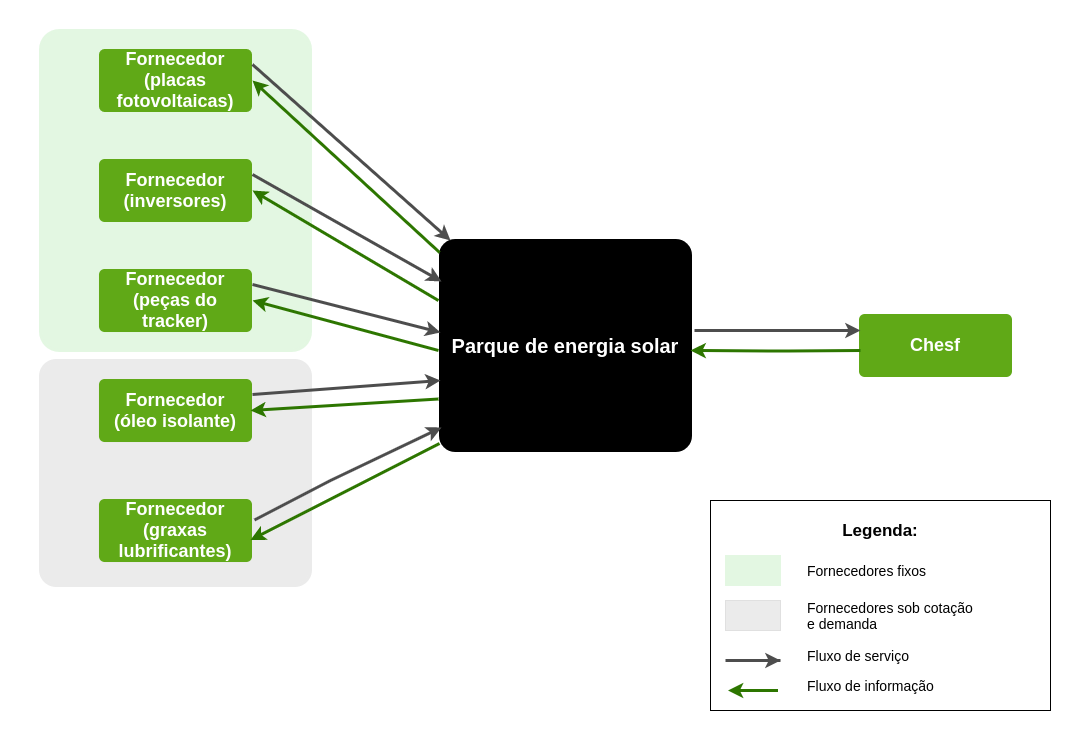
\includegraphics[scale=0.48]{images/cadeia_suprimentos_sunburn.png}
    \caption*{Fonte: Autoria própria.}
    \label{fig:cadeia_suprimentos_sunburn}
\end{figure}
  

